% Created by tikzDevice version 0.12.3.1 on 2021-12-04 14:30:11
% !TEX encoding = UTF-8 Unicode
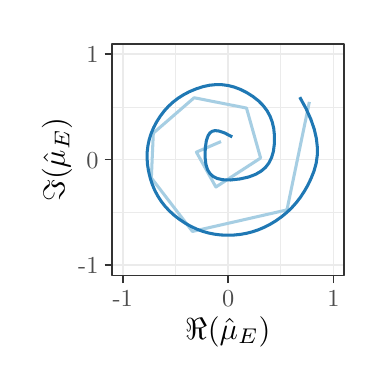
\begin{tikzpicture}[x=1pt,y=1pt]
\definecolor{fillColor}{RGB}{255,255,255}
\begin{scope}
\definecolor{drawColor}{RGB}{255,255,255}
\definecolor{fillColor}{RGB}{255,255,255}

\path[draw=drawColor,line width= 0.6pt,line join=round,line cap=round,fill=fillColor] (  0.22,  0.00) rectangle (119.75,119.97);
\end{scope}
\begin{scope}
\definecolor{fillColor}{RGB}{255,255,255}

\path[fill=fillColor] ( 30.47, 30.69) rectangle (114.25,114.47);
\definecolor{drawColor}{gray}{0.92}

\path[draw=drawColor,line width= 0.3pt,line join=round] ( 30.47, 53.54) --
	(114.25, 53.54);

\path[draw=drawColor,line width= 0.3pt,line join=round] ( 30.47, 91.62) --
	(114.25, 91.62);

\path[draw=drawColor,line width= 0.3pt,line join=round] ( 53.32, 30.69) --
	( 53.32,114.47);

\path[draw=drawColor,line width= 0.3pt,line join=round] ( 91.40, 30.69) --
	( 91.40,114.47);

\path[draw=drawColor,line width= 0.6pt,line join=round] ( 30.47, 34.49) --
	(114.25, 34.49);

\path[draw=drawColor,line width= 0.6pt,line join=round] ( 30.47, 72.58) --
	(114.25, 72.58);

\path[draw=drawColor,line width= 0.6pt,line join=round] ( 30.47,110.66) --
	(114.25,110.66);

\path[draw=drawColor,line width= 0.6pt,line join=round] ( 34.27, 30.69) --
	( 34.27,114.47);

\path[draw=drawColor,line width= 0.6pt,line join=round] ( 72.36, 30.69) --
	( 72.36,114.47);

\path[draw=drawColor,line width= 0.6pt,line join=round] (110.44, 30.69) --
	(110.44,114.47);
\definecolor{drawColor}{RGB}{166,206,227}

\path[draw=drawColor,line width= 1.1pt,line join=round] ( 69.78, 79.11) --
	( 60.89, 75.30) --
	( 67.93, 62.69) --
	( 84.09, 73.16) --
	( 78.99, 91.22) --
	( 60.08, 94.95) --
	( 45.32, 82.16) --
	( 44.61, 65.97) --
	( 59.46, 46.64) --
	( 76.53, 50.53) --
	( 93.61, 54.42) --
	( 97.66, 73.93) --
	(101.71, 93.44);
\definecolor{drawColor}{RGB}{31,120,180}

\path[draw=drawColor,line width= 1.1pt,line join=round] ( 73.83, 80.80) --
	( 71.06, 82.24) --
	( 69.06, 82.92) --
	( 67.63, 83.07) --
	( 66.59, 82.83) --
	( 65.78, 82.25) --
	( 65.09, 81.21) --
	( 64.50, 79.49) --
	( 64.10, 76.82) --
	( 64.02, 73.46) --
	( 64.32, 70.85) --
	( 64.93, 68.93) --
	( 65.80, 67.53) --
	( 66.94, 66.50) --
	( 68.45, 65.76) --
	( 70.47, 65.32) --
	( 73.18, 65.23) --
	( 76.67, 65.61) --
	( 79.80, 66.32) --
	( 82.29, 67.27) --
	( 84.27, 68.42) --
	( 85.85, 69.77) --
	( 87.09, 71.37) --
	( 88.04, 73.27) --
	( 88.71, 75.57) --
	( 89.07, 78.36) --
	( 89.10, 81.27) --
	( 88.83, 83.86) --
	( 88.29, 86.18) --
	( 87.50, 88.29) --
	( 86.43, 90.23) --
	( 85.09, 92.04) --
	( 83.42, 93.74) --
	( 81.38, 95.36) --
	( 79.04, 96.84) --
	( 76.74, 97.99) --
	( 74.51, 98.82) --
	( 72.30, 99.38) --
	( 70.10, 99.67) --
	( 67.87, 99.69) --
	( 65.58, 99.46) --
	( 63.20, 98.94) --
	( 60.73, 98.13) --
	( 58.39, 97.15) --
	( 56.25, 96.03) --
	( 54.29, 94.78) --
	( 52.48, 93.40) --
	( 50.81, 91.87) --
	( 49.27, 90.18) --
	( 47.85, 88.31) --
	( 46.54, 86.26) --
	( 45.41, 84.11) --
	( 44.51, 81.97) --
	( 43.84, 79.83) --
	( 43.38, 77.67) --
	( 43.12, 75.48) --
	( 43.06, 73.23) --
	( 43.21, 70.90) --
	( 43.59, 68.47) --
	( 44.18, 65.99) --
	( 44.93, 63.68) --
	( 45.83, 61.52) --
	( 46.90, 59.50) --
	( 48.12, 57.60) --
	( 49.51, 55.81) --
	( 51.09, 54.10) --
	( 52.86, 52.48) --
	( 54.84, 50.95) --
	( 56.87, 49.60) --
	( 58.92, 48.45) --
	( 60.99, 47.49) --
	( 63.09, 46.70) --
	( 65.23, 46.09) --
	( 67.44, 45.65) --
	( 69.72, 45.37) --
	( 72.08, 45.27) --
	( 74.46, 45.34) --
	( 76.75, 45.57) --
	( 78.98, 45.96) --
	( 81.15, 46.52) --
	( 83.29, 47.24) --
	( 85.40, 48.13) --
	( 87.49, 49.20) --
	( 89.57, 50.46) --
	( 91.61, 51.90) --
	( 93.52, 53.46) --
	( 95.29, 55.15) --
	( 96.93, 56.98) --
	( 98.45, 58.95) --
	( 99.86, 61.08) --
	(101.17, 63.38) --
	(102.36, 65.88) --
	(103.43, 68.58) --
	(104.18, 71.34) --
	(104.57, 74.17) --
	(104.59, 77.12) --
	(104.24, 80.22) --
	(103.49, 83.53) --
	(102.27, 87.09) --
	(100.55, 90.95) --
	( 98.25, 95.14);
\definecolor{drawColor}{gray}{0.20}

\path[draw=drawColor,line width= 0.6pt,line join=round,line cap=round] ( 30.47, 30.69) rectangle (114.25,114.47);
\end{scope}
\begin{scope}
\definecolor{drawColor}{gray}{0.30}

\node[text=drawColor,anchor=base east,inner sep=0pt, outer sep=0pt, scale=  0.88] at ( 25.52, 31.46) {-1};

\node[text=drawColor,anchor=base east,inner sep=0pt, outer sep=0pt, scale=  0.88] at ( 25.52, 69.55) {0};

\node[text=drawColor,anchor=base east,inner sep=0pt, outer sep=0pt, scale=  0.88] at ( 25.52,107.63) {1};
\end{scope}
\begin{scope}
\definecolor{drawColor}{gray}{0.20}

\path[draw=drawColor,line width= 0.6pt,line join=round] ( 27.72, 34.49) --
	( 30.47, 34.49);

\path[draw=drawColor,line width= 0.6pt,line join=round] ( 27.72, 72.58) --
	( 30.47, 72.58);

\path[draw=drawColor,line width= 0.6pt,line join=round] ( 27.72,110.66) --
	( 30.47,110.66);
\end{scope}
\begin{scope}
\definecolor{drawColor}{gray}{0.20}

\path[draw=drawColor,line width= 0.6pt,line join=round] ( 34.27, 27.94) --
	( 34.27, 30.69);

\path[draw=drawColor,line width= 0.6pt,line join=round] ( 72.36, 27.94) --
	( 72.36, 30.69);

\path[draw=drawColor,line width= 0.6pt,line join=round] (110.44, 27.94) --
	(110.44, 30.69);
\end{scope}
\begin{scope}
\definecolor{drawColor}{gray}{0.30}

\node[text=drawColor,anchor=base,inner sep=0pt, outer sep=0pt, scale=  0.88] at ( 34.27, 19.68) {-1};

\node[text=drawColor,anchor=base,inner sep=0pt, outer sep=0pt, scale=  0.88] at ( 72.36, 19.68) {0};

\node[text=drawColor,anchor=base,inner sep=0pt, outer sep=0pt, scale=  0.88] at (110.44, 19.68) {1};
\end{scope}
\begin{scope}
\definecolor{drawColor}{RGB}{0,0,0}

\node[text=drawColor,anchor=base,inner sep=0pt, outer sep=0pt, scale=  1.10] at ( 72.36,  7.64) {$\Re(\hat\mu_E)$};
\end{scope}
\begin{scope}
\definecolor{drawColor}{RGB}{0,0,0}

\node[text=drawColor,rotate= 90.00,anchor=base,inner sep=0pt, outer sep=0pt, scale=  1.10] at ( 13.30, 72.58) {$\Im(\hat\mu_E)$};
\end{scope}
\end{tikzpicture}
